\section{Experiments}

\subsection{Input data}
To test the correctness of the algorithms we used the MONK's datasets. To use these datasets correctly we did the following steps:
\begin{itemize}
	\item We preprocessed MONK's datasets with \textit{1-of-k} encoding to convert categorical data to numerical data and we obtained 17 binary input features vectors. This preprocessing is divided between two classes, \textit{Preprocessing} and \textit{LoadDataset}. The former reads, shuffle and split the dataset whereas the latter performs the \textit{1-to-k} encoding. 
	\item To view all the network in vector formulation terms and exploit the \textit{Armadillo} numerical library, we performed batch computation by loading and transposing the entire dataset in a single matrix. The labels were split and saved in another matrix to compute the \textit{MSE} (sez \ref{Loss:Mse}) after the forward phase. To reduce the cost of moving matrices we took advantage of the \textit{move} operator available since C++11. 
	\item Our library can deal with classification and regression tasks exploiting the composition of the \textit{Layer} class.  So we implemented \textit{sigmoid} and \textit{linear} activation functions for the output layer and \textit{hyperbolic tangent} activation function for the hidden layers.
\end{itemize}


\subsection{MONKS} 
To obtain a deterministic behaviour of the algorithms, we used the entire MONKS datasets as the input of the network. We obtained three matrices that had dimensions: 124x18 (Monk 1), 169x17 (Monk 2), and 122x17 (Monk 3). To compare the behaviour of the algorithms, we collected three parameters for every epoch: the error of the network (in our case MSE), the norm of the gradient and the computational time spent on completing the epoch. These three parameters were used to make the convergence speed, residual and computational time plots shown below. For better visualization of the plots an enlargement of each of them is shown aside. Before showing the plots a table with all the configurations used and the values obtained is shown.

\begin{center}
	\small\addtolength{\tabcolsep}{-3pt}
		\centering
		\begin{longtable}{|c|c|c|c|c|c|c|c|c|}
			\hline
			\textbf{Task}& \textbf{Optimizer}&\textbf{Iteration} & \textbf{L rate} & \multicolumn{1}{l|}{\textbf{Lambda}} & \textbf{Mom} & \textbf{MSE}& \textbf{$\Vert \nabla f_{k}\Vert$ }& \textbf{Time(ms)}\\ \hline 
			Monk1 & MDA & 900 & 0.9 & 0  & 0 & 8.67e-3 & 3.450e-1 & 267 \\
			Monk1 & MDA & 900 & 0.9 & 0  & 0.3 & 2.458e-3 & 1.390e-1 & 231 \\
			Monk1 & MDA & 900 & 0.9 & 0  & 0.6 & 7.535e-4 & 5.0557e-1 & 233 \\
			Monk1 & MDA & 900 & 0.9 & 0  & 0.9 & 1.159e-4 & 8.59058e-3 & 405 \\
			Monk1 & NMDA & 900 & 0.9 & 0  & 0 & 8.678e-2 & 3.450e-1 & 279 \\
			Monk1 & NMDA & 900 & 0.9 & 0  & 0.3 & 2.426e-3 & 1.381-e1 & 265 \\
			Monk1 & NMDA & 900 & 0.9 & 0  & 0.6 & 7.472e-4 & 5.093e-1 & 222 \\
			Monk1 & NMDA & 900 & 0.9 & 0  & 0.9 & 1.124e-4 & 8.992e-3 & 208 \\
			Monk1 & L-BFGS & 50 & - & 0  & 0 & 11e-15 & 784e-13 & 3267 \\
			Monk1 & L-BFGS & 50 & - & 3e-4  & 0 & 6.396e-2 & 1.134e-1 & 3623 \\
			Monk1 & L-BFGS & 50 & - & 5e-4  & 0 & 8.553e-2 & 9.089e-1 & 3733 \\
			Monk1 & L-BFGS & 50 & - & 7e-4  & 0 & 1.201e-1 & 1.245e-1 & 5943 \\
			Monk1 & PBM & 400 & - & 0  & 0 & 6.962e-6 & 7.510e-4 & 29642 \\
			Monk1 & PBM & 400 & - & 3e-4  & 0 & 8.114e-1 & 7.510e-4 & 26849 \\
			Monk1 & PBM & 400 & - & 5e-4  & 0 & 1.352e-1 & 7.510e-4 & 27618 \\
			Monk1 & PBM & 400 & - & 7e-4  & 0 & 1.893e-1 & 7.510e-4 & 28247 \\
			Monk2 & MDA & 900 & 0.9 & 0  & 0 & 7.946e-2 & 5.151e-1 & 148\\
			Monk2 & MDA & 900 & 0.9 & 0  & 0.3 & 2.374e-2 & 3.236e-1 & 1128 \\
			Monk2 & MDA & 900 & 0.9 & 0  & 0.6 & 1.332e-2 & 8.083e-2 & 119 \\
			Monk2 & MDA & 900 & 0.9 & 0  & 0.9 & 6.673e-4 & 3.102e-2 & 342\\
			Monk2 & NMDA & 900 & 0.9 & 0  & 0 & 7.946e-2 & 5.151e-1 & 116\\
			Monk2 & NMDA & 900 & 0.9 & 0  & 0.3 & 2.486e-2 & 3.802e-1 & 179\\
			Monk2 & NMDA & 900 & 0.9 & 0  & 0.6 & 1.380e-2 & 9.093e-2 & 116\\
			Monk2 & NMDA & 900 & 0.9 & 0  & 0.9 & 1.403e-4 & 1.382e-2 & 939\\
			Monk2 & L-BFGS & 50 & - & 0  & 0 & 7.6e-14 & 3.788e-12 & 5610\\
			Monk2 & L-BFGS & 50 & - & 3e-4  & 0  & 5.919e-2 & 9.413e-2 & 5324\\
			Monk2 & L-BFGS & 50 & - & 5e-4  & 0  & 1.156e-1& 4.682e-1 & 6142\\
			Monk2 & L-BFGS & 50 & - & 7e-4  & 0  & 8.965e-2 &  4.468e-1 & 10047\\
			Monk2 & PBM & 400 & - & 0  & 0 & 3.453e-6 & 3.365e-4 & 37746\\
			Monk2 & PBM & 400 & - & 3e-4  & 0 & 1.211e-1 & 3.365e-4 & 37129\\
			Monk2 & PBM & 400 & - & 5e-4  & 0 & 2.018e-1 & 3.365e-4 & 39902\\
			Monk2 & PBM & 400 & - & 7e-4  & 0 & 2.825e-1 & 3.365e-4 & 37130\\
			Monk3 & MDA & 900 & 0.9 & 0  & 0 & 1.968e-2 & 3.236e-2 & 280\\
			Monk3 & MDA & 900 & 0.9 & 0  & 0.3 & 1.864e-2 & 2.297e-2 & 131\\
			Monk3 & MDA & 900 & 0.9 & 0  & 0.6 & 1.754e-2 & 1.301e-2 & 105\\
			Monk3 & MDA & 900 & 0.9 & 0  & 0.9 & 1.254e-2 & 7.248e-3 & 142\\
			Monk3 & NMDA & 900 & 0.9 & 0  & 0 & 1.968e-2 & 3.236e-2 & 106\\
			Monk3 & NMDA & 900 & 0.9 & 0  & 0.3 & 1.863e-2 & 2.277e-2 & 129\\
			Monk3 & NMDA & 900 & 0.9 & 0  & 0.6 & 1.754e-2 & 1.267e-2 & 300\\
			Monk3 & NMDA & 900 & 0.9 & 0  & 0.9 & 1.254e-2 & 7.139e-3 & 189\\
			Monk3 & L-BFGS & 50 & - & 0  & 0 & 8.196e-3 & 1.068e-12 & 8319\\
			Monk3 & L-BFGS & 50 & - & 3e-4  & 0  & 5.781e-2 & 3.603e-1 & 7947\\
			Monk3 & L-BFGS & 50 & - & 5e-4  & 0  & 8.555e-2 & 1.895e-1 & 12729\\
			Monk3 & L-BFGS & 50 & - & 7e-4  & 0  & 7.940e-2 & 1.525e-1 & 10153\\
			Monk3 & PBM & 400 & - & 0  & 0 & 1.231e-2 & 8.410e-4 & 35543\\
			Monk3 & PBM & 400 & - & 3e-4  & 0 & 7.988e-2 & 8.410e-4 & 35239\\
			Monk3 & PBM & 400 & - & 5e-4  & 0 & 1.249e-1 & 8.410e-4 & 35924\\
			Monk3 & PBM & 400 & - & 7e-4  & 0 & 1.699e-1 & 8.410e-4 & 35003\\
			\hline
			\caption{Network configurations with MSE.}
			\label{tab:nets_res}
		\end{longtable}

\end{center}

\subsubsection{Residual}
The residual values results we obtained from the algorithms respect what we expect from the theory.  As we can see from the plots below (see fig \ref{R-Monk1} for example), the number of epochs needed to convergence by the L-BFGS confirms the superlinear convergence behaviour we mentioned above (sez. \ref{L-BFGSConv}).  Also we can see in the plots that the linear convergence of the Momentum Descent Approach (sez.  \ref{MDA-convergence}) and the Proximal Bundle Method (sez. \ref{PBM-Convergence}) is respected. Of course, the curves obtained from the Proximal Bundle Method are not smooth as those obtained with the Momentum Descent Approach, this is because Bundle methods construct and minimize an approximation $f_B(x)$ of the function using the subgradients (as mention above sez. \ref{Bundle-methods}).  It's interesting to view that all of these methods even with a noisy dataset as Monk 3 converge with the same convergence rate as mentioned in the theory.

\begin{figure}[H]
	\centering
	\begin{minipage}[t]{0.5\linewidth}
		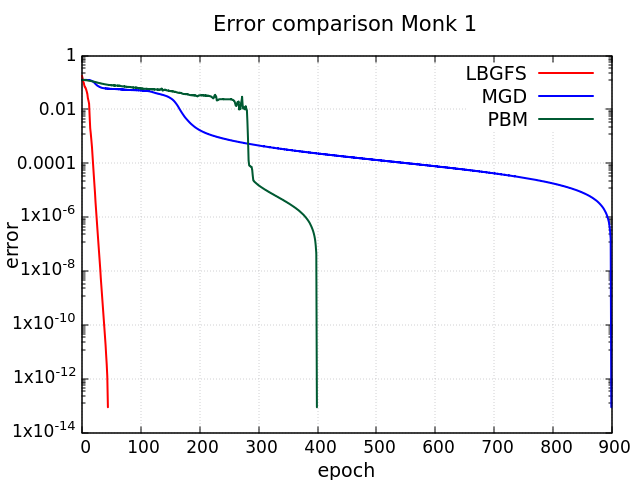
\includegraphics[width=\linewidth]{data/Comparison/Monk1/Monk1_R_Comparison_log_standard.png}
		%\subcaption{MSE}
	\end{minipage}%
	\begin{minipage}[t]{0.5\linewidth}
		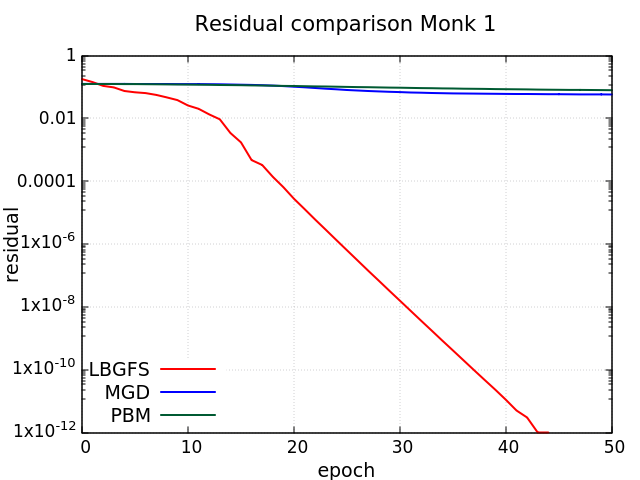
\includegraphics[width=\linewidth]{data/Comparison/Monk1/Monk1_R_Comparison_log_zoom.png}
		%\subcaption{Accuracy}
	\end{minipage}
	\caption{Residual comparison Monk 1}
	\label{R-Monk1}
\end{figure}
\begin{figure}[H]
	\centering
	\begin{minipage}[t]{0.5\linewidth}
		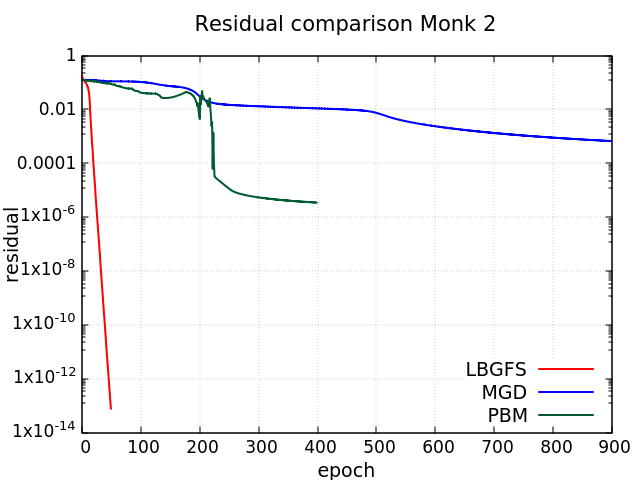
\includegraphics[width=\linewidth]{data/Comparison/Monk2/Monk2_R_Comparison_log_standard.png}
		%\subcaption{MSE}
	\end{minipage}%
	\begin{minipage}[t]{0.5\linewidth}
		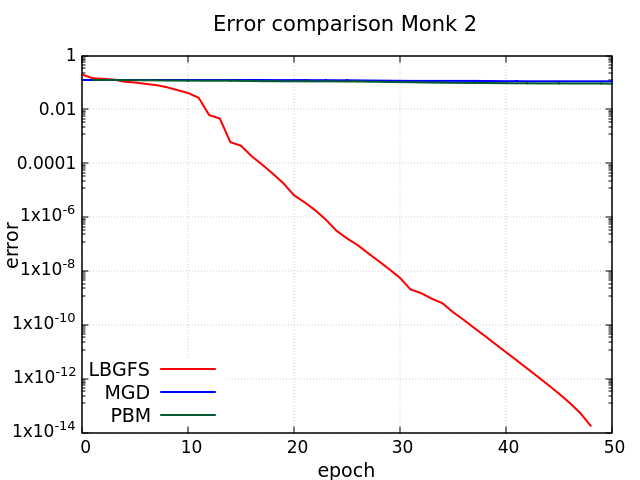
\includegraphics[width=\linewidth]{data/Comparison/Monk2/Monk2_R_Comparison_log_zoom.png}
		%\subcaption{Accuracy}
	\end{minipage}
	\caption{Residual comparison Monk 2}
	\label{R-Monk2}
\end{figure}
\begin{figure}[H]
	\centering
	\begin{minipage}[t]{0.5\linewidth}
		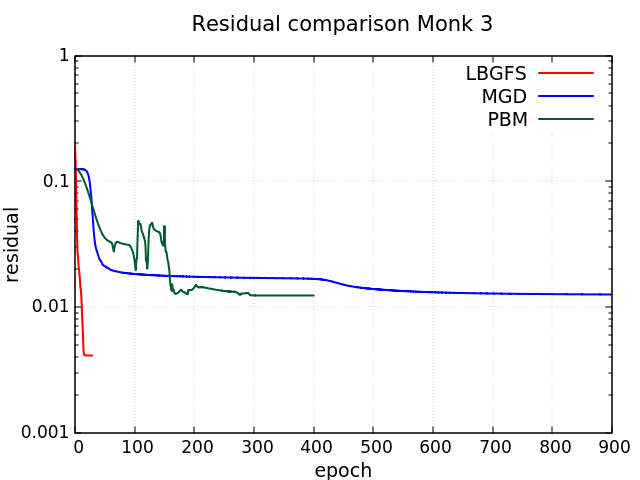
\includegraphics[width=\linewidth]{data/Comparison/Monk3/Monk3_R_Comparison_log_standard.png}
		%\subcaption{MSE}
	\end{minipage}%
	\begin{minipage}[t]{0.5\linewidth}
		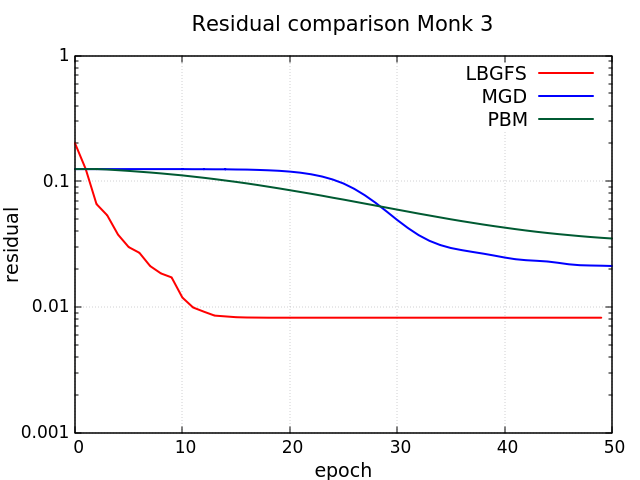
\includegraphics[width=\linewidth]{data/Comparison/Monk3/Monk3_R_Comparison_log_zoom.png}
		%\subcaption{Accuracy}
	\end{minipage}
	\caption{Residual comparison Monk 3}
	\label{R-Monk3}
\end{figure}
\subsubsection{Computational time}
To compare the computational time behaviour of the implemented algorithm, we decided to display their curves in the plots \ref{CT-Monk1},\ref{CT-Monk2}, and \ref{CT-Monk3}. We can observe that, as expected from the theory, the most expensive method is the Proximal Bundle Method because of the time spent on the resolution of a quadratic programming problem by an external solver. As we can see in table \ref{tab:nets_res} the computational time of the Momentum Descent Approach is always lower than the others, it means that it is faster to reach a good value of the error in the Monks dataset. Moreover, we can infer that the L-BFGS algorithm gives us the best approximation of the objective function, meanwhile at a greater cost for each iteration. This is due to the better descent direction given by the approximation of the Hessian. Also, for this approximation, it has to pay some high computational costs that usually do not allow to use this kind of approach in all the situation. 

\begin{figure}[H]
	\centering
	\begin{minipage}[t]{0.5\linewidth}
		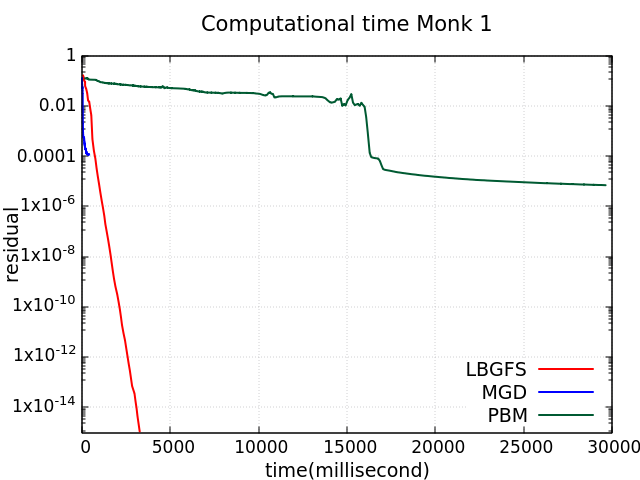
\includegraphics[width=\linewidth]{data/Comparison/Monk1/Monk1_CT_Comparison_log_standard.png}
		%\subcaption{MSE}
	\end{minipage}%
	\begin{minipage}[t]{0.5\linewidth}
		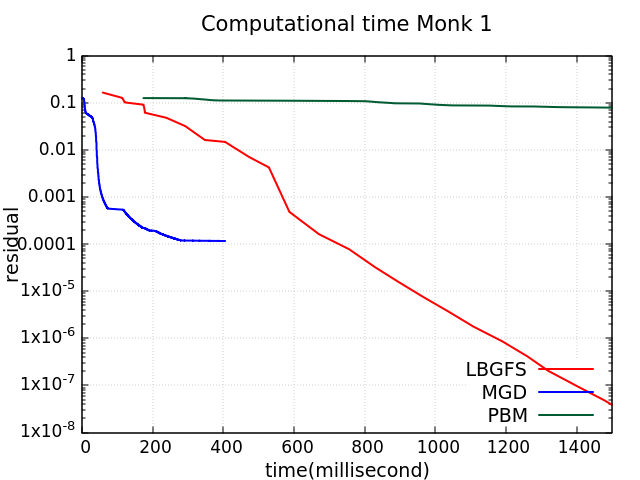
\includegraphics[width=\linewidth]{data/Comparison/Monk1/Monk1_CT_Comparison_log_zoom.png}
		%\subcaption{Accuracy}
	\end{minipage}
	\caption{Computational time comparison Monk 1}
	\label{CT-Monk1}
\end{figure}
\begin{figure}[H]
	\centering
	\begin{minipage}[t]{0.5\linewidth}
		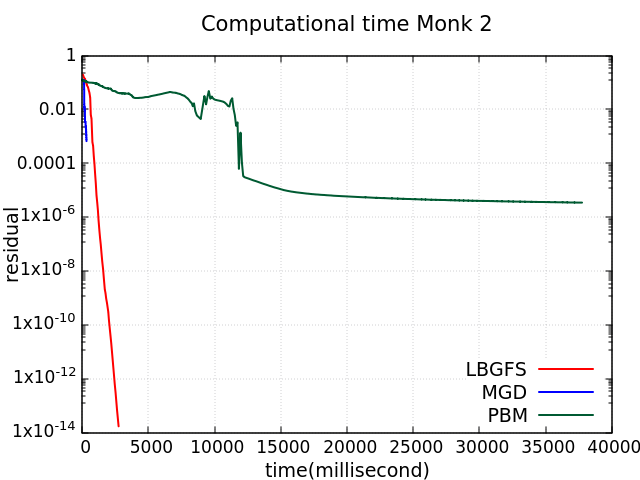
\includegraphics[width=\linewidth]{data/Comparison/Monk2/Monk2_CT_Comparison_log_standard.png}
		%\subcaption{MSE}
	\end{minipage}%
	\begin{minipage}[t]{0.5\linewidth}
		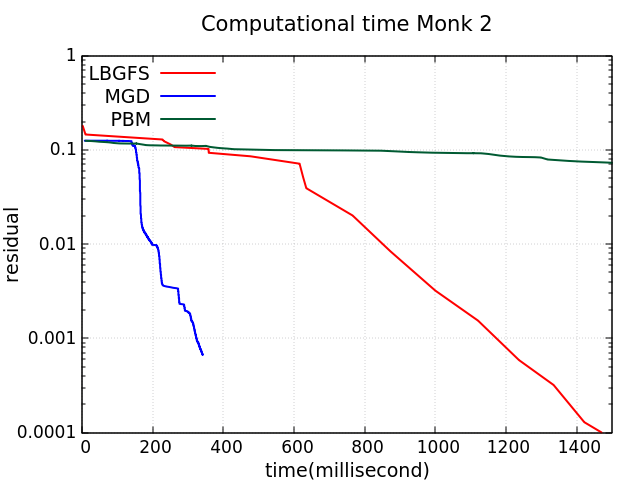
\includegraphics[width=\linewidth]{data/Comparison/Monk2/Monk2_CT_Comparison_log_zoom.png}
		%\subcaption{Accuracy}
	\end{minipage}
	\caption{Computational time comparison Monk 2}
	\label{CT-Monk2}
\end{figure}
\begin{figure}[H]
	\centering
	\begin{minipage}[t]{0.5\linewidth}
		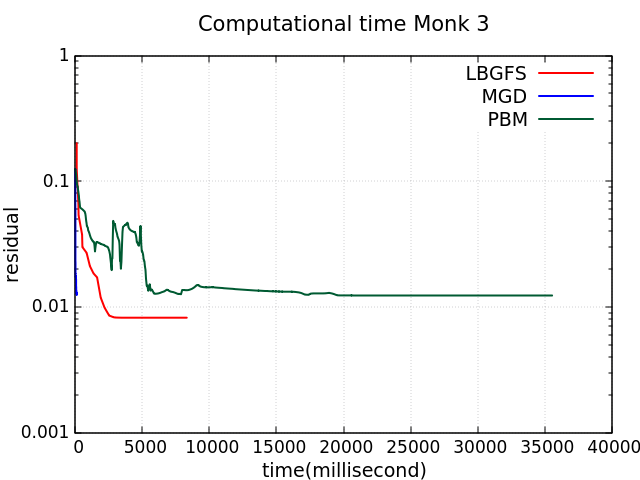
\includegraphics[width=\linewidth]{data/Comparison/Monk3/Monk3_CT_Comparison_log_standard.png}
		%\subcaption{MSE}
	\end{minipage}%
	\begin{minipage}[t]{0.5\linewidth}
		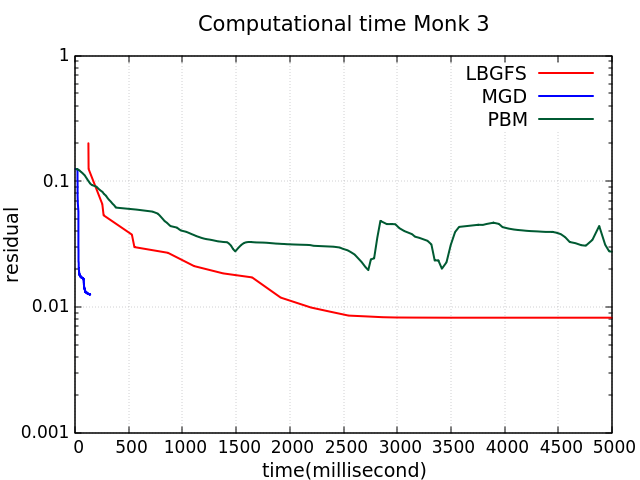
\includegraphics[width=\linewidth]{data/Comparison/Monk3/Monk3_CT_Comparison_log_zoom.png}
		%\subcaption{Accuracy}
	\end{minipage}
	\caption{Computational time comparison Monk 3}
	\label{CT-Monk3}
\end{figure}



\subsubsection{Gradient norm convergence speed}
Here we can observe that the behaviour of the algorithms follows what we stated before in the theory about their convergence speed. We view from the plots that the norm of the gradient is not smooth in all the Monks dataset. In our opinion, this is due to the starting point of the training and the non-convexity of the objective function. We know from the theory that these methods tend to have some problems with the local minimum. Also, we can observe that at a certain point the norm tends to stabilize and converge to zero. Therefore, we can infer that in the neighbourhood of the last visited minima there are no other minimum better than itself and the search of the best minima can stop.
\begin{figure}[H]
	\centering
	\begin{minipage}[t]{0.5\linewidth}
		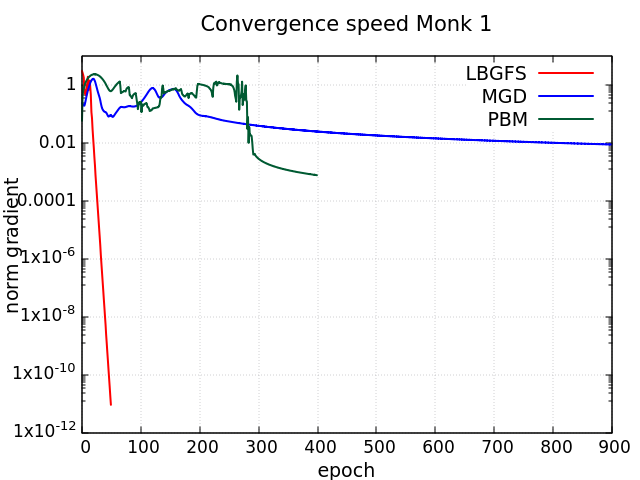
\includegraphics[width=\linewidth]{data/Comparison/Monk1/Monk1_CS_Comparison_log_standard.png}
		%\subcaption{MSE}
	\end{minipage}%
	\begin{minipage}[t]{0.5\linewidth}
		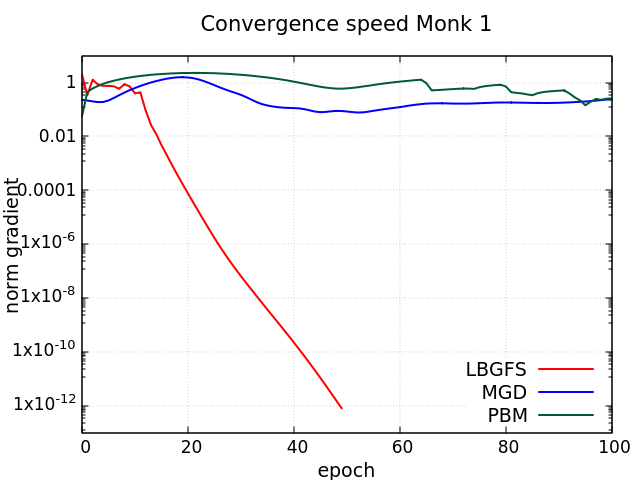
\includegraphics[width=\linewidth]{data/Comparison/Monk1/Monk1_CS_Comparison_log_zoom.png}
		%\subcaption{Accuracy}
	\end{minipage}
	\caption{Converge speed comparison Monk 1}
	\label{CS-Monk1}
\end{figure}
\begin{figure}[H]
	\centering
	\begin{minipage}[t]{0.5\linewidth}
		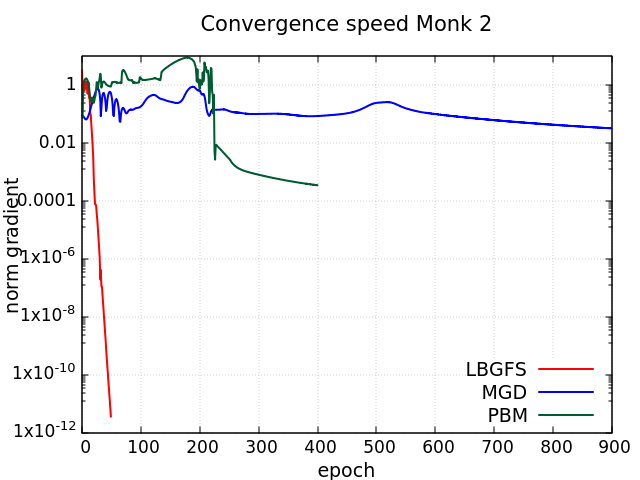
\includegraphics[width=\linewidth]{data/Comparison/Monk2/Monk2_CS_Comparison_log_standard.png}
		%\subcaption{MSE}
	\end{minipage}%
	\begin{minipage}[t]{0.5\linewidth}
		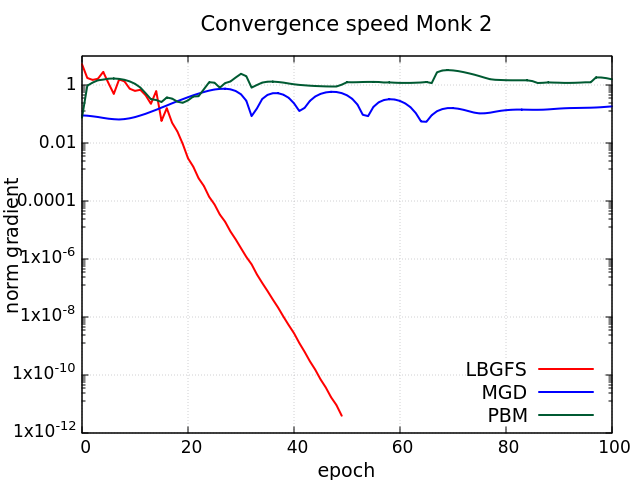
\includegraphics[width=\linewidth]{data/Comparison/Monk2/Monk2_CS_Comparison_log_zoom.png}
		%\subcaption{Accuracy}
	\end{minipage}
	 \caption{Converge speed comparison Monk 2}
	 \label{CS-Monk2}
\end{figure}
\begin{figure}[H]
	\centering
	\begin{minipage}[t]{0.5\linewidth}
		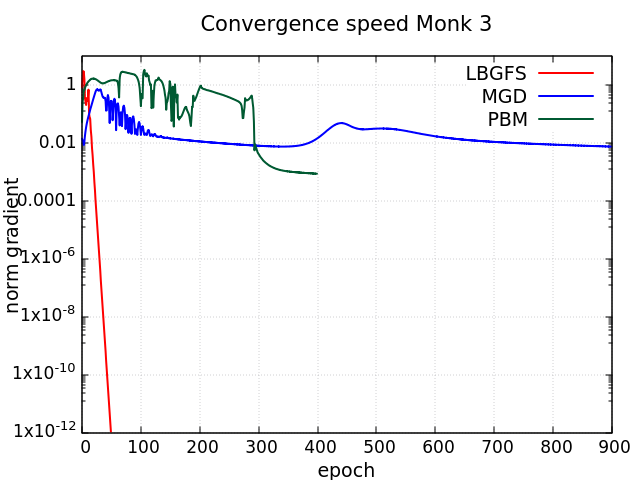
\includegraphics[width=\linewidth]{data/Comparison/Monk3/Monk3_CS_Comparison_log_standard.png}
		%\subcaption{MSE}
	\end{minipage}%
	\begin{minipage}[t]{0.5\linewidth}
		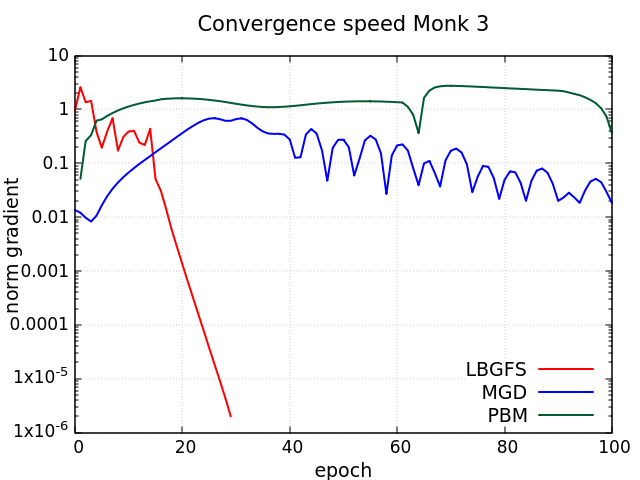
\includegraphics[width=\linewidth]{data/Comparison/Monk3/Monk3_CS_Comparison_log_zoom.png}
		%\subcaption{Accuracy}
	\end{minipage}
	\caption{Converge speed comparison Monk 3}
	\label{CS-Monk3}
\end{figure}

\subsection{Conclusions on the experiments}
As said in \S\ref{LF:convexity}, the objective function is not convex. For this reason, we try to understand if the methods analysed were approaching the same minima or different ones. First of all, the analysis and comparisons were made on the weights of each different network. We observed that only the Proximal Bundle Method was convergent to the same minima for each different hyperparameters configurations. Also, we had examined the others network, and we found that there are some minima near each other and for this reason, the weights of the network sometimes do not differ too much (e.g. Momentum Descent Approach with 0.3 and 0.6 of classical momentum with Monk1 dataset). After further analysis, we observed that the weights initialization definitely influences the choice of the minima.